%%%%%%%%%%%%%%%%
% Latex Vorlage \includegraphics[]{Bakkarbeit.pdf}
% zum Schreiben einer Bakk.-Arbeit
%%%%%%%%%%%%%%%%


% Load all the Headers that are needed 

%%%%%%%%%%%%%%%%%%%
% Latex Headers for Bakkarbeit.tex
%%%%%%%%%%%%%%%%%%%


\documentclass [12pt, a4paper, bibtotocnumbered, liststotocnumbered, normalheadings]{scrartcl}
\usepackage[latin9]{inputenc}
\usepackage[english]{babel}

% Graphiken einbinden
\usepackage{graphicx}
\usepackage{float}

% Anklickbare Links im PDF file
\usepackage{url}
\usepackage[pdftex, bookmarks, bookmarksopen=true, bookmarksnumbered=true]{hyperref}

% Glossary
\usepackage[nonumberlist]{glossaries}
\makeglossaries

\newglossaryentry{A}{name={A}, description={Infection by Airbourne}}
\newglossaryentry{ACAT}{name={ACAT}, description={\textbf{A}ge \textbf{C}are \textbf{A}ssessment \textbf{T}eam}}
\newglossaryentry{AD}{name={AD}, description={\textbf{A}s \textbf{D}esired Diet (anything the patients wants to eat)}}
\newglossaryentry{AIN}{name={AIN}, description={\textbf{A}ssistant \textbf{i}n \textbf{N}ursing}}
\newglossaryentry{AMO}{name={AMO}, description={\textbf{A}ccredited \textbf{M}edical \textbf{O}fficer}}
\newglossaryentry{Analgesia}{name={Analgesia}, description={pain medication}}
\newglossaryentry{Anti-emetic}{name={Anti-emetic}, description={medication against nausea}}
\newglossaryentry{Arthroplasty}{name={Arthroplasty}, description={plastic surgery of a joint}}
\newglossaryentry{B}{name={B}, description={\textbf{B}owels}}
\newglossaryentry{BD}{name={BD}, description={twice a day}}
\newglossaryentry{BGL}{name={BGL}, description={\textbf{B}lood \textbf{G}lucose \textbf{L}evel}}
\newglossaryentry{Bolus}{name={Bolus}, description={a rounded mass of food or pharmaceutical preparation ready to swallow, or such a mass passing through the gastrointestinal tract}}
\newglossaryentry{BP}{name={BP}, description={\textbf{B}lood \textbf{P}ressure}}
\newglossaryentry{BSL}{name={BSL}, description={\textbf{B}lood \textbf{S}ugar \textbf{L}evel}}
\newglossaryentry{C}{name={C}, description={infection by contact}}
\newglossaryentry{CF}{name={CF}, description={\textbf{C}lear \textbf{F}luids}}
\newglossaryentry{CMO}{name={CMO}, description={\textbf{C}areer \textbf{M}edical \textbf{O}fficer (doctor on call)}}
\newglossaryentry{Comorbidity}{name={Comorbidity}, description={other illnesses that a patient has that are not part of the diagnosis but affect the health of the patient and possibly the treatment (ie. Diabetes, Hypertension)}}
\newglossaryentry{Cont}{name={Cont}, description={\textbf{C}ontinence (bowels)}}
\newglossaryentry{CVC}{name={CVC}, description={\textbf{C}entral \textbf{V}enus \textbf{C}atheter}}
\newglossaryentry{D}{name={D}, description={infection by droplet}}
\newglossaryentry{DW}{name={DW}, description={\textbf{D}ry \textbf{W}eight (weight of patient before breakfast)}}
\newglossaryentry{Dx}{name={Dx}, description={diagnosis}}
\newglossaryentry{EDD}{name={EDD}, description={\textbf{E}stimated \textbf{D}ate of \textbf{D}ischarge}}
\newglossaryentry{EEN}{name={EEN}, description={\textbf{E}ndorsed \textbf{E}nrolled \textbf{N}urse. Have completed further medication endorsement. Allowed to administer Schedule 2,3, and 8 medications via all routes except intravenous, epidural, intraventriuclar and intrathecal. Any medication which requires checking prior to administration must be checked with a RN or Midwife. Excluded also from administering fluids or medications via CVC, PICC and femoral lines as well implanted devices or arterial lines}}
\newglossaryentry{EN}{name={EN}, description={\textbf{E}nrolled \textbf{N}urse. Nurses undertook 18/24 month course at TAFE or related health facilities). Even more restricted than EEN}}
\newglossaryentry{FF}{name={FF}, description={\textbf{F}ull \textbf{F}luids incl. milky drinks}}
\newglossaryentry{HITH}{name={HITH}, description={\textbf{H}ospital \textbf{i}n \textbf{t}he \textbf{H}ome}}
\newglossaryentry{Hx}{name={Hx}, description={history}}
\newglossaryentry{iCIMS}{name={iCIMS}, description={\textbf{i}ntegrated \textbf{C}linical \textbf{I}nformation \textbf{M}anagement \textbf{S}ystem. A design application developed at the University of Sydney allowing the creation of information systems without the necessity of programming experience}}
\newglossaryentry{IDC}{name={IDC}, description={\textbf{I}n-\textbf{D}welling \textbf{C}atheter}}
\newglossaryentry{IM}{name={IM}, description={\textbf{I}ntra\textbf{m}uscular (routed into muscle tissue)}}
\newglossaryentry{IVC/F}{name={IVC/F}, description={\textbf{I}ntravenous \textbf{C}annula (a catheter that is inserted into a vein for supplying medications or nutrients directly into the bloodstream) / \textbf{I}ntravenous \textbf{F}luids (fluids given through a vein inserted catheter}}
\newglossaryentry{L}{name={L}, description={Light Diet}}
\newglossaryentry{LOS}{name={LOS}, description={\textbf{L}ength \textbf{o}f \textbf{S}tay of a patient}}
\newglossaryentry{MO}{name={MO}, description={\textbf{M}edical \textbf{O}fficer}}
\newglossaryentry{MRN}{name={MRN}, description={\textbf{M}edical \textbf{R}ecord \textbf{N}umber}}
\newglossaryentry{MRO}{name={MRO}, description={\textbf{M}ethacilin \textbf{R}esistant \textbf{O}rganism; an organism that shows resistance to Methicillin, a very strong antibiotic}}
\newglossaryentry{MRSA}{name={MRSA}, description={\textbf{M}ulti \textbf{R}esistant \textbf{S}taphylococcus \textbf{A}ureus; any strain of Staphylococcus aureus that has developed resistance to beta-lactam antibiotics, which include the penicillins (methicillin, dicloxacillin, nafcillin, oxacillin, etc.)}}
\newglossaryentry{N}{name={N}, description={Neutropenic (very low white blood cell count). Caution must be taken by staff as they could pass something to a patient}}
\newglossaryentry{NBM}{name={NBM}, description={\textbf{N}il \textbf{B}y \textbf{M}outh}}
\newglossaryentry{NCR}{name={NCR}, description={\textbf{N}urse \textbf{C}are \textbf{R}ecord}}
\newglossaryentry{ND}{name={ND}, description={night shift}}
\newglossaryentry{NFR}{name={NFR}, description={\textbf{N}ot \textbf{F}or \textbf{R}esuscitation}. The patient does not want the clinical staff to use life saving measures}
\newglossaryentry{NG}{name={NG}, description={\textbf{N}asal-\textbf{G}astric Tube}}
\newglossaryentry{NP}{name={NP}, description={\textbf{N}urse \textbf{P}ractitioner is a RN educated and authorised to function autonomously and collaboratively in an advanced and extended clinical role. Requires addition 1.5-2 years of study}}
\newglossaryentry{NUM}{name={NUM}, description={\textbf{N}ursing \textbf{U}nit \textbf{M}anager}}
\newglossaryentry{OT}{name={OT}, description={\textbf{O}ccupational \textbf{T}herapist}}
\newglossaryentry{PAC}{name={PAC}, description={\textbf{P}ressure \textbf{A}rea \textbf{C}are}}
\newglossaryentry{Palliative}{name={Palliative}, description={relieving or soothing the symptoms of a disease or disorder with effecting a cure}}
\newglossaryentry{PEG}{name={PEG}, description={\textbf{P}ercutaneous \textbf{E}ndoscopic \textbf{G}astrostomy tube; tube that is inserted into the stomach to give nutrition}}\newglossaryentry{PICC}{name={PICC}, description={\textbf{P}eripherally \textbf{I}nserted \textbf{C}entral \textbf{C}atheter}}
\newglossaryentry{PRN}{name={PRN}, description={as required medication; these are not part of the patients regular medications)}}
\newglossaryentry{QID}{name={QID}, description={four times a day}}
\newglossaryentry{RN}{name={RN}, description={\textbf{R}egistered \textbf{N}urse. a graduate nurse who has been legally authorized (registered) to practice after examination by a state board of nurse examiners or similar regulatory authority, and who is legally entitled to use the designation RN.}}
\newglossaryentry{Rx}{name={Rx}, description={treatment pertaining to medication / subscriptions}}
\newglossaryentry{S}{name={S}, description={strict precaution (Infection Risk)}}
\newglossaryentry{SC}{name={SC}, description={\textbf{S}hower \textbf{C}omode (in chair)}}
\newglossaryentry{SC Fluids}{name={SC Fluids}, description={\textbf{S}ub\textbf{c}utaneous Fluids; fluids administered just under the skin and not into a vein}}
\newglossaryentry{SH}{name={SH}, description={shower}}
\newglossaryentry{SP}{name={SP}, description={sponge bath in bed}}
\newglossaryentry{SPC}{name={SPC}, description={\textbf{S}upra \textbf{P}ubic \textbf{C}atheter}}
\newglossaryentry{ST}{name={ST}, description={shower with trolley}}
\newglossaryentry{TB}{name={TB}, description={\textbf{T}owel \textbf{B}ath}}
\newglossaryentry{TDS}{name={TDS}, description={three times a day}}
\newglossaryentry{TEDS}{name={TEDS}, description={brand of Anti-embolic Stockings that are used to prevent blood clots}}
\newglossaryentry{TKVO}{name={TKVO}, description={\textbf{T}o \textbf{K}eep \textbf{V}ein \textbf{O}pen}}
\newglossaryentry{TL}{name={TL}, description={\textbf{T}eam \textbf{L}eader}}
\newglossaryentry{TPN}{name={TPN}, description={\textbf{T}otal \textbf{P}arenteral \textbf{N}utrition; all nutrition is given through a catheter}}
\newglossaryentry{Trainee Consultant/Registrar}{name={Trainee Consultant/Registrar}, description={doctor learning his or her speciality}}
\newglossaryentry{U}{name={U}, description={\textbf{U}rine \textbf{OR} MRO Risk (Unknown Status) mean a risk assumption has been made but not proven}}
\newglossaryentry{VTE}{name={VTE}, description={\textbf{V}enous \textbf{T}hrombo\textbf{e}mbolism; i.e. blood clot in the vein}}
\newglossaryentry{Warfarin}{name={Warfarin}, description={anticoagulant medicine; nurses need to be aware of patients receiving this due to higher risk of bleeding and in case of bleeds}}


% PDF Titel, Autor etc setzen:
\hypersetup{
	pdftitle={Gathering and Designing a Multi-Disciplinary Surgical  Clinical Ward Handover System at the SAN Hospital},
	pdfauthor={Patrick Mumme},
}

% Seite einrichten
\usepackage{geometry}
\geometry{verbose, a4paper, tmargin=2cm, bmargin=1.7cm, lmargin=2cm, rmargin=2cm, headsep=0cm}

% Zeilenabstand
\usepackage{setspace}
\setstretch{1.3}

% Kopf- und Fusszeilen
\usepackage{fancyhdr}
\pagestyle{fancy}
\headheight33pt
\headsep1cm
\footskip1cm
\textheight23cm

\lhead{
\includegraphics[height=1cm]{Images/usyd_logo}}
\chead{} 
\rhead{\nouppercase{\leftmark}} 

\lfoot{SANSURGIMS} 
\cfoot{} 
\rfoot{Page \thepage} 

% Zitate aus Bibtex Bibliographien
%\usepackage[square, authoryear, sort]{natbib}
% \bibliographystyle{plainnat}
\usepackage[square, authoryear]{natbib}
\bibliographystyle{apa}

%\usepackage[style=apa]{natlib}
%\usepackage{csquotes}

% Tabellen 
\usepackage{tabularx} % fuer einseitige tabellen
\usepackage{supertabular} % mehrseitige tabellen

% Source Code Listings
\usepackage{listings} 
\lstset{
  float,
  basicstyle=\small, 
  tabsize=2, 
  numbers=left, 
  numberstyle=\tiny, 
  numbersep=5pt, 
  frame=lines, 
  breaklines=false,
  prebreak={\mbox{\ensuremath{\hookleftarrow}}},
  postbreak={\space\space},
  breakindent=0pt,
  captionpos=b
}


% Kommentare
% Damit kann man \begin{comment}...\end{comment} verwenden!
\usepackage{comment}
\usepackage{fancybox}
\newenvironment{commentenvironment}% 
{\begin{Sbox}\begin{minipage}}% 
{\end{minipage}\end{Sbox}\shadowbox{\TheSbox}} 
\specialcomment{comment}
{\begin{commentenvironment}{\textwidth}}
{\end{commentenvironment}}

% Alle Kommentare ausblenden geht so:
%\excludecomment{comment}


% Aufzaehlungen mit enumerate
\usepackage{enumerate}


% Lyx Listen f�r Kompatibilit�t mit Lyx Quellcode
\newenvironment{lyxlist}[1]
{\begin{list}{}
{\settowidth{\labelwidth}{#1}
 \setlength{\leftmargin}{\labelwidth}
 \addtolength{\leftmargin}{\labelsep}
 \renewcommand{\makelabel}[1]{##1\hfil}}}
{\end{list}}


% Verhinderung von "Schusterjungen"
% einzelne Absatzzeilen auf der Seite unten
\clubpenalty = 10000

% Verhinderung von "Hurenkindern"
% einzelne Zeilen eines Absatzes am Kopf der Seite
\widowpenalty = 10000





% Begin with the document
\begin{document}


% Titelseite
\begin{titlepage}

\pagestyle{empty}
%\noindent

\setstretch{1}

    	\begin{figure}[hp]
				\centering
				
\includegraphics[scale=1.0, width=70mm]{Images/usyd_logo}
	\end{figure} 
			
\bigskip

\begin{center}
    \Huge\bfseries
   Gathering and Designing a Multi-Disciplinary Surgical  Clinical Ward Handover System at the SAN Hospital
\end{center}
\begin{center}
    \Large
    Patrick Mumme \\
   310262135
\end{center}
\bigskip

\begin{center}
\Large
COMP5703 \\
Information Technologies Project \\
Semester 1, 2012\\
\bigskip\bigskip\bigskip
under the direction of\\
Prof. Jon Patrick \\
June 12th, 2012
\end{center}


\bigskip


\vspace*{\fill}

\cleardoublepage

\rmfamily
\normalfont

\end{titlepage}

%Abstract
\addcontentsline{toc}{section}{Abstract}
\begin{center}
\Large\bfseries
Surgical Ward Clinical Handover System
\end{center}

\section*{Abstract}
A hospital is a labyrinth of paper forms and corridor communication. In order to find their way, users must use considerable effort in order to receive and transfer information. The information system SANSURGIMS aims to make it considerably easier to access this information. Through requirements analysis and system design, the student has created a system that allows clinical staff to more efficiently transfer information from one shift to the next. This not only makes their work easier but also allows them to spend more time doing their real work, taking care of patients. 

\section*{Acknowledgements}
I would like to thank the Sydney Adventist Hospital for giving me the chance to experience a living, breathing hospital setting. I would like to thank Chris Williams for making these projects possible. I would like to thank Hannah Chong for her guidance and support during my stay at the hospital. She helped me stay afloat in the sea of information that is patient care. I would like to thank Vivien Lane and Jane Gardner as well as the many other staff at the SAN that spared their time to review and guide my work. I would also like to thank Janelle Craig for helping me to settle into the SAN. I would like to thank Prof. Jon Patrick and Decler Hague for their academic support and guidance through this project. I would like to thank Prof. Jon Patrick for giving me the opportunity to work with iCIMS.


% Table of Contents
\newpage{}
\tableofcontents{}
\setcounter{tocdepth}{5}
\newpage{}

%Glossary

\phantomsection
\addcontentsline{toc}{section}{Glossary}
\glsaddall
\printglossary


% Chapters
\section{Introduction}
\subsection{Client Profile}
Originally opened in Wahroonga on January 1 1903 as a 70 bed Sanitarium, the Sydney Adventist Hospital (SAH), known to the local residents as `The San', is a not-for-profit hospital of the South Pacific Division of the Seventh-day Adventist Church.  Today, the hospital is a private hospital offering acute care and currently has 358 licensed overnight beds. SAH is the largest single campus private hospital within NSW and was the first of its kind to be accredited by the Australian Council on Healthcare Standards. SAH is proud to have won the Australian Private Hospitals Association Award for Clinical Excellence in the category 70 beds and over in 2006.
 \\ \\
The San prides itself on being the single biggest employer within the Hornsby-Kuring-gai area employing over 2,200 staff and around 700 accredited medical practitioners. Together, the SAN staff care for more than 50,000 inpatients and about 160,000 outpatients. The San is also known for its maternity wards and is proud to be bringing over 2,000 babies a year into the world. The SAN, being one of few private hospitals to offer emergency care, admits over 20,000 patients annually making it NSW's largest and busiest emergency care department among private hospitals. The SAN offers medical services ranging from acute surgical, medical and obstetric care to complex cardiac and orthopaedic procedures. The SAN boasts cutting edge facilities that include a dozen operation theatre suites, 3 state-of-the-art Cardiac Catheterisation Laboratories and Australia's first dual source CT scanner. The SAN is also responsible for operating the San Day Surgery Hornsby and Dalcross Adventist Hospital, located in Killara.
\\ \\
With the mission statement ``Christianity in Action", the SAN not only offers world class care to the patients within the hospital, but also to disadvantaged third world men, women and children as part of its HealthCare Outreach program. Since its inception in 1986, the HealthCare Outreach program has undertaken 100 trips to 13 different countries culminating in over 2,800 surgeries and lives saved. 
\newpage

\subsection{Project Description and Scope}
\subsubsection{Project Description}
The SAN Hospital Information System has to service many different clinical specialities and environments. This project will develop a prototype application in the form of a simulator of a novel HIT system for surgical patients. These patients typically have specific and predictable post-surgical outcomes and hospitalisation time-frames, as outlined in various surgical clinical pathways (e.g. Urology such as, Greenlight Laser Prostatectomy, Ear, Nose and Throat (ENT) and Plastics). Caring for these patients requires information systems for multidisciplinary nursing and allied health staff.
Constructing a requirements document will be a complex task but give students the richest possible experience in understanding all the stages of requirements gathering, systems design and systems implementation. The project will use a research technology simulator that enables the process of requirements gathering and system design to be integrated as a single process and thereby enable validation of requirements by their implementation into a design simulator. 

\subsubsection{Scope}
The project will commence with the gathering of requirements by meeting and interviewing various clinical staff fulfilling a variety of roles on the surgical ward, level 11. The student will also gather all paper based forms in use on the ward as references during the design process. Upon completion of the first phase of requirements gathering, a requirements document will be created and will represent the basis for design decisions. Throughout the rest of the semester the student will update the requirements document as necessary. The student will design forms, including the clinical handover, in the simulator as well as obtain end user feedback during the majority of the semester. Towards the end of the semester, the student will undertake user acceptance testing as well as evaluations of the work done. The project will conclude with a first draft of the clinical handover form and a presentation to SAN staff. The project will finish at the end of the academic semester.

\newpage
\subsection{Project Objectives}
\label{Project Objectives}
\begin{itemize}
\item Collect the requirements for a Clinical Handover for use by nurses, allied health and medical staff in the care of surgical patients
\item Produce an accurate record of the information each worker needs access to in the form of a requirements document including process flows
\item Design and develop a prototype which simulates an electronic clinical information system with handover processes for nurses, doctors and other clinical staff
\end{itemize}

\subsubsection{Risks}

\begin{tabular}{|l|l|l|l|l|}
\hline
{\bf Ref \#} & {\bf Probability} & {\bf Impact} & {\bf Description} & {\bf Mitigation} \\
\hline
R.1 & High & Medium & Reduced performance through & Increase allotted tool  \\ & & & use of new technology & usage time  \\ 
\hline
R.2 & Low & High & Unable to complete project  & frequent comm- \\ & & & objectives due to simulator & unication with \\ & & & issues & simulator developers  \\  
\hline
R.3 & Medium & Medium & Scope creep & Clearly outline scope \\ & & & &  at outset of project \\
\hline
\end{tabular}

\subsubsection{Assumptions}

\begin{tabular}{|l|l|l|}
\hline
{\bf Ref \#} & {\bf Description} \\
\hline
A.1 & The simulator will not need to connect to existing SAN applications \\
\hline
A.2 & We will have access to a simulator developer \\
\hline
A.3 & A project manager will be available to assist us in our work at the hospital \\ 
\hline
A.4 & We are not developing a system for actual use \\
\hline
\end{tabular}

\subsubsection{Issues}

\begin{tabular}{|l|l|l|l|}
\hline
{\bf Ref \#} & {\bf Priority} & {\bf Description} & {\bf Owner} \\
\hline
I.1 & High & Simulator bugs \& issues & Simulator Developer \\
\hline
I.2 & Medium & Exposed to immense amount of information & Student \\
\hline
I.3 & Medium & Sporadic staff availability  & Student \& PM \\
\hline
I.4 & Low & Time constraints due to university courses & Student \\
\hline
\end{tabular}


\newpage
\subsection{Anticipated Outcomes / Results for the Project}
\subsubsection{First Draft Computerised Handover Form}
At the conclusion of this project, the student should have designed a first draft of a computerised handover form. This draft does not need to contain all information required but should focus on the most important pieces of information especially in regards to nurses. It should convey all relevant design decisions and be capable of representing patients with varying degrees of complexity, the degree to which a patient is ill.

\subsubsection{Understanding of IT/IS within the Health Domain}
The student will have gained a general understanding of not only the health domain but also the role of IT IS systems within a hospital setting. The student should see the advantages of using computerised information systems to support the clinical staff in their daily work.
 
 \subsubsection{Requirements Analysis Complete}
By the end of the semester, the student should have completed the requirements analysis for the project. This should include all relevant requirements up to the end of the academic semester. As part of the requirements analysis, the student should have created as-is and to-be process diagrams for the nurse to nurse handover.

\subsubsection{Design of a Simulation of the Desired System}
A designer tool was to be used to create a simulation of the information system that conformed to the collected requirements. The simulation will have been assessed by clinical staff for its conformance to the expressed requirements.

\subsection{Benefits of the Project}
\subsubsection{Technology Evangelisation}
Through the project, the student will be able to show the advantages and abilities of computerised information systems to clinical staff, in particular nursing staff. Although the clinical staff at the SAN are using applications to record information already, not all aspects of their daily work are digitised including handover. By working with staff throughout the semester, the student will be able to generate end-user buy-in and support for a computerised clinical handover.

\newpage
\subsubsection{Pilot Project}
This project constitutes a pilot project in the sense that future students can build upon the achievements of this project. The foundation, both in regard to system design as well as end-user exposure, will provide future students with a lower entry barrier into the clinical domain and into the SAN.

\subsubsection{End-User Driven Development}

The project will expose the student to a new development methodology model in conjunction with a design tool. This will provide the student with the opportunity to compare and contrast traditional development methodologies with this newly created model. 

\subsubsection{Trialing the Designer Tool}
This project allowed the student to use a health information system application called \gls{iCIMS} which is intended for creating a simulator of the ideal system for the user. The project can thus be seen as a trial for the designer tool enabling the student to not only use a new technology but also to document bugs and suggest enhancements to the system. In essence, the student ran the application through its paces and noted shortcomings as well as possible additional features allowing the application to go through a maturation process. 
\section{Process}
\subsection{Overview}
\label{Overview}
In order to take full advantage of the tools employed in this project as well as the opportunity to work at the hospital, an iterative and incremental user driven development process was chosen. This allowed the student to take advantage of the tacit knowledge of clinical staff and allowed the end-user to actively participate in the design of the system. The iterative and incremental nature of the process allowed the student to start with one form and then incrementally add more forms as well as managing iterative changes in existing forms through user feedback. The ultimate goal of any project is to supply an outcome that will be accepted by the stakeholders, in this case the end users. User driven development enabled the designer to ensure that during all steps in the project the system met stakeholder needs and requirements. The active feedback gained from clinical staff enabled the designer to shape and form the system to meet user needs. It is important to note that sitting down with clinical staff was not always possible as their priority lies with patient care. In order to facilitate a continued design process throughout the semester a number of methods were employed. The student utilised participative observations, interviews as well as feedback notes to gain an adequate understanding of the user needs and requirements. The student's work at the SAN was supported by a project manager from the SAN, Hannah Chong, that facilitated first meetings with clinical staff as well as offering feedback on relevant project management aspects of the project.

\subsubsection{Participative Observations}
As this was the first time the designer had undertaken a IT project within the health domain it was important to learn how clinical staff worked. Participative observations facilitated this need through \emph{shadowing} clinical staff during various points in their shift. This included sitting in on clinical handover, the process through which the nurse of the previous shift conveys patient information to the nurses of the oncoming shift. By sitting in on handover the designer was able to gain an understanding of the overall process of clinical handover as well as experience the shortcomings and inefficiencies first hand. This enabled the designer to relate to the clinical staff when discussing the system design. 
\\ \\
The designer did not actively participate in handover, that is to say that the designer merely observed and did not give handover. Thus, the designer acted like a `fly on the wall', remaining in the background looking on. This method proved vital to the project as it provided a first hand experience of the current situation. One disadvantage of using participative observations was that the designer was overwhelmed at first by the sheer amount of information that he was exposed to. It took some time and effort on the part of the designer to sift through, filter and understand the information in order to make the most efficient use of it. As the project progressed this information overload continually decreased.

\subsubsection{User Interviews}
In order to supplement participative observations, user interviews were undertaken with various clinical staff fulfilling different roles within the hospital. This enabled the designer to understand the viewpoints of various staff in regards to what they do as well as their view on clinical handover. The interviews lasted between ten and fifteen minutes and were held casually. During the interviews, the designer asked specific questions about handover and the user's involvement. The interviews were held on the ward or in offices depending on the role of the staff being interviewed. The interviews also served the purpose of building a relationship with the clinical staff. The designer's aim was to go back to the interviewed staff throughout the project and attain their feedback on the system design. This social component was very important in order to elicit staff support especially nursing staff as their time was extremely limited. Not undertaking this social component would have made the work of the designer much more difficult.

\subsubsection{Feedback Notes}
During the course of the project, the designer met with clinical staff at various times in order to show them the current status of the design as well as to get answers to open questions. During each of these encounters, notes were taken in order to preserve the exchange allowing the designer to return to the notes at a later time to refresh his memory. In order to maximise the use of time with the clinical staff the designer was accompanied by a colleague who assisted with taking notes during the feedback sessions. This allowed the designer to focus on the staff and not waste time trying to write down information as well as facilitating a smooth flow during the meetings with staff.

\newpage
\subsection{Tools and Skills}
From the beginning of the project, one of the key aspects was the use of the \gls{iCIMS}.  Having been created recently, the project was meant to trial the tool in a real world scenario. The main ideology behind iCIMS is to use a graphical interface to build a system thus avoiding the necessity for programming skills. This means that end-users could actively participate in designing the system by creating the system together with the designer. iCIMS aims to be applicable in any clinical situation and thus utilises Ockham's Razor of Design (\cite{Budd}), which states that :

\begin{quote}
\center\emph{``a design should use the minimal number of entities \\ with their maximal generalisations"}
\end{quote}
\vspace{6mm}
\noindent In conjunction with using iCIMS, the designer utilised Trac, a bug and issue tracking system that also offers documentation functionality in the form of a wiki. Two separate instances of Trac were used because the iCIMS project had an existing instance. All bugs and issues were documented in the iCIMS instance of Trac and all project documentation was created in a separate instance of Trac available for the project. All relevant project information, such as interview notes, process flows, etc., was documented on the Trac instance. Apart from playing a vital role in the completion of the project academically, the wiki will also serve as a starting point for future designers continuing the project. This ensures that the designer's efforts are properly recorded and will allow future designers to more easily find their way on future projects.
\\ \\
Apart from electronic tools, the designer needed to use communication and people skills in order to successfully undertake this project. Communication and people skills played a vital role as the designer was dealing with end-users that were very technology-adverse as well as having a low computer-literacy. Inter-personal skills allowed the designer to find common ground and terminology with which to communicate with end-users. It also allowed the designer to quell most reservations that clinical staff had towards the project or its purpose.

\newpage
\subsection{Scope and Schedule}
Although the project description outlines that the designer undertake a design of the entire multi-disciplinary handover occurring at the SAN, this was deemed too big of a scope to handle within an academic semester. Figure \ref{Clinical Handover Overview - All User Roles} is a depiction that hints at the complexity and size of the entire clinical handover process.

\begin{figure}[hp]
				\centering
				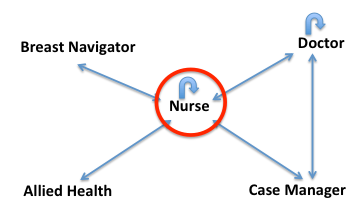
\includegraphics[scale=1.0, width=80mm]{Images/Clinical_Handover_All_Roles}
				\caption{Clinical Handover Overview - All User Roles}
				\label{Clinical Handover Overview - All User Roles}
\end{figure} 

\noindent As shown in figure \ref{Clinical Handover Overview - All User Roles}, there are numerous roles involved in clinical handover each with their own needs and requirements. It was deemed infeasible to undertake requirements analysis, system design and evaluation for all clinical staff involved. The sheer amount of information, communication complexity as well as immense design effort lead to the decision to focus on the nurse role for this project, denoted by the red circle in the figure above. Furthermore, the scope was defined as focusing on the clinical handover between nurses as this was deemed most important in discussions with staff. The nurse to nurse handover is also the most structured handover between clinical staff lending itself to be best suited to this project. 

\newpage 
\noindent With regards to scheduling, the project was divided into four major phases as depicted in figure \ref{Project Process and Schedule}. The week numbers are based on the academic semester timeframe.

\begin{figure}[hp]
				\centering
				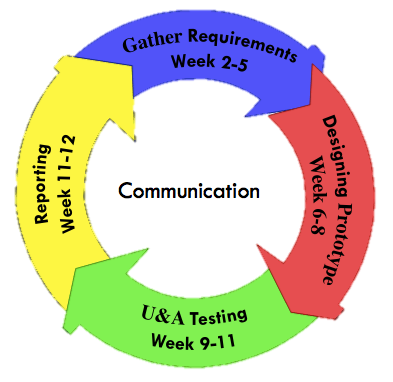
\includegraphics[scale=1.0, width=80mm]{Images/Project_Process}
				\caption{Project Process and Schedule}
				\label{Project Process and Schedule}
\end{figure} 

\noindent Even though the project was divided into four phases, all phases were undertaken in parallel at most times. The separation merely depicts where the focus lay at each point in time. The schedule of four weeks for requirements gathering was a good estimate and allowed the designer to perform an adequate analysis thus enabling the designer to proceed to the design phase. The design phase's projected timeframe of three weeks was too short and was actually the focus of the designer's work until week twelve. This stems from the fact that the designer had numerous issues with the design tool in the form of bugs and it also took longer than expected to convert design ideas into reality within the design tool. This principally because the designer was not familiar with the design tool or its components prior to commencing the project.
\\ \\
Due to the extensive design phase, the usability and acceptance testing phase was pushed back into the weeks twelve and thirteen after the designer was at a point in the design that lent itself to such testing. Although the testing phase timeframe was reduced to two weeks and pushed to the very end of the academic semester, the designer nevertheless managed to obtain testing data in coordination with staff. Due to availability issues with staff, not all clinical staff could undertake the usability and acceptance testing. It should be noted that these availability issues did not stem from bad time or appointment management on behalf of the designer, but rather on issues surrounding staff being sick or having to take personal days off. 
\\ \\
The last phase, the reporting phase, was the focus of week thirteen of the project having been pushed back in order to allow for usability and acceptance testing. This did not pose a major issue as the majority of the reporting phase was in the form of the academic report. The other portion of the reporting phase where the weekly status meetings with Prof. Jon Patrick and the documentation of information in the wiki throughout the semester. At the centre of all phases and indeed of the project lay the communication with clinical staff as well as the project manager Hannah Chong and Prof. Jon Patrick.

\section{SANSURGIMS}


\section{Evaluation}
During the course of the project, feedback was repeatedly sought from clinical staff in regards to the progression of SANSURGIMS. This feedback was not only valuable to the student in regard to designing but also necessary in order to ensure continued alignment with requirements and staff needs. Towards the end of the project, this staff feedback was complimented with a questionnaire in order to attain quantifiable values that would lend themselves to analysis. The student's view of SANSURGIMS was not included in any evaluation because end-users make much better judges when used in conjunction with measurement instruments as they, the end-users, tend to see things more in regards to strategic benefits for the organisation as opposed to the more system-benefit centric view of an IS professional (\cite{MiraniLederer}). This leads to an overarching statement of IS Success and is said best by \cite{Seddon}:

\begin{quote}
\center\emph{``IS Success is [...] conceptualized as a value judgement made by an individual, from the point of some stakeholder."}
\end{quote}
\vspace{6mm} 
 
\subsection{Testing Procedures}
As mentioned above, the evaluation of the system was undertaken in two forms. The first form of evaluation, direct user feedback, was utilised during the majority of the project lifespan. The student met with clinical staff repeatedly and presented them with the current system. The student was accompanied by another student during these feedback sessions that was responsible for assisting in note taking. This way, the student was able to give the clinical staff his full attention and facilitate a constructive session. 
\\ \\
The second form of evaluation undertaken was the use of a questionnaire at the end of the project (Appendix \ref{Clinical Handover Questionnaire}). The questionnaire first asked the clinical staff member to navigate to the handover for a specific patient and then answer specific questions about that patient. The task was used to determine how well the user could navigate the system and if he or she could find information in an acceptable time frame. After completing the small tasks, the clinical staff usually gave feedback in regard to the handover form on their own accord. After their feedback was noted, the clinical staff member was asked to answer the questions on the questionnaire. The objective of the questionnaire was to present the staff member with a small number of questions to which the he or she only needed to circle the statement that most corresponded with their view. It was very important that the questionnaire be short and easy to fill out in order to not give the clinical staff the feeling that reviewing the system was a very time consuming matter. This plays an important role in regards to obtaining subsequent feedback. If staff feel that reviewing the system is too time consuming they might refrain from giving feedback.

\subsection{Test Results}

The continual feedback received from various clinical staff included a range of responses. These ranged from being very positive about the work being done to citing short comings of SANSURGIMS or even misconceptions introduced by the student. The feedback was always perceived as constructive and the student believes that these responses were earnest views of the system. 
\\ \\
In regards to the questionnaire, the responses were mostly positive. There were some issues with navigating the system where clinical staff did not see the handover button on the right side of the table and instead opted to click on the row within the table. Others were uncertain when using the system and paused for one to two seconds before clicking the button. A third group of users were more confident in using the system and did not hesitate. The questions in the tasks were answered in a timely manner for the most part with only one user taking considerably longer to find the information. This stemmed from the fact that the user was taking longer to orientate themselves within the system than other users. The average rating in the questionnaire by question is displayed below:

\begin{figure}[hp]
				\centering
				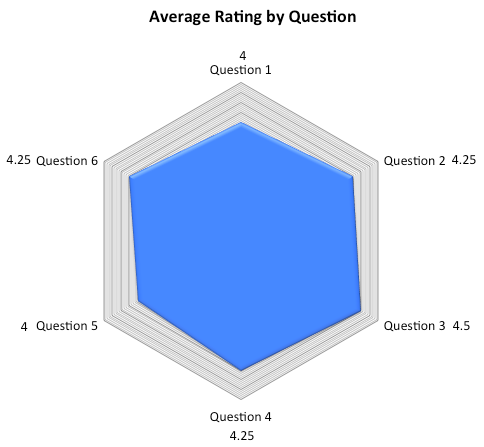
\includegraphics[scale=1.0, width=80mm]{Images/Evaluation-Results}
				\caption{Questions Results - Averaged}
\end{figure}

\newpage
\subsection{Interpretation of Results}
While staff feedback was viewed as earnest and constructive in regards to SANSURGIMS, it nevertheless needs to be taken with a grain of salt. This stems from the fact that there are numerous influences acting on a stakeholder and each will affect how the stakeholder views and acts during the project. In regards to the clinical staff, one could argue that time pressures and the fact that they were not consulted on whether to have such a project be undertaken on their ward or not lead to a lack of full support. The staff was very helpful, but the amount of support might have been greater if staff were able to allocate some of their time to SANSURGIMS. This of course is quite difficult to achieve given the nature of the staff's work. The feedback given still allowed the student to design a system that was received positively by the staff.
\\ \\
The positive reception by staff is further supported by the results of the questionnaire questions as depicted above. All questions, on average, were answered with a score of 4 and above. This means that there was no information overload, it was easy to find information, the information had a logical order, the colours were informative, SANSURGIMS would increase handover efficiency and the system was easy to navigate. There is one caveat to the positive results of the questionnaire; the student was only able to have four members of clinical staff fill out the questionnaire. This was due to time constraints on the part of the student as well as the staff and unforeseen personal circumstances ranging sick staff to staff not being available for an extended period of time due to their absence from the hospital. The small sample size greatly weakens the proposition of the results, that SANSURGIMS is meeting staff needs and requirements effectively. That is not to say that the opposite is true, but there is no objective proof to support that conclusion at this point in time. 
\\ \\
Even though the testing and validation measures are lacking, the student still believes that a system was built that meets staff requirements and would serve the goals of a digital handover. SANSURGIMS can be viewed as a successful pilot project into this domain and has potential that warrants a continuation of the work by other students.
\\ \\ 
The strengths of the work lie within building a relationship with the staff and introducing them to a digital information system in which they hold the power to make decisions. It allowed a good portion of the clinical staff to come to the realisation that a digital handover would make their work easier and cause them less headaches in terms of the quality of handover and the medium through which it is communicated. 
\\ \\
The weakness of the system is that it focused on aggregating information into a handover form and thus neglected data entry. Forms were created for data entry, but these were only created as a first draft version and not continually updated. These forms were not directly shown to staff all the time, but all were shown at least once. The forms served merely as a way to adequately design the handover form. This also meant that no evaluation was undertaken on these forms due to the fact that they were first drafts as well as time constraints. 
\\ \\
The reasoning behind this choice was that the data entry was more of a pre-requisite rather than an integral part of the actual handover, the main part of the project. Another reason why the data aggregation was favoured was because the surgical ward was already utilising another application for most of its work documentation. If implemented on the ward, SANSURGIMS would integrate with that application and pull the data from there rather than from forms created within SANSURGIMS. Thus, the student chose to make a strategic long term decision during the design phase that would position SANSURGIMS in such a way as to mitigate redundant design should it ever be integrated into the ward.

\section{Future Work}

\section{Reflection}
\subsection{Contribution}


\subsection{Difficulties}

\subsection{Lessons Learned}

\subsection{Future Suggestions}

\section{Conclusion}
\subsection{Concluding Remarks}


\subsection{Strengths and Weaknesses}

\subsection{A Second Time}


\subsection{Future Work}


% Appendizes
\appendix





% Literaturverzeichnis
\renewcommand{\refname}{Bibliography} 
\nocite{*} %this needs to be here in order to get the Bilbiography to show without having cited
\bibliography{bib/References}

\section{Appendix}

Include the following:
\begin{itemize}
\item Roles at SAN wiki page
\item Scans of original questionnaires
\item Screenshots of SANSURGIMS (Web and Designer)
\item Scans of important forms (Nursing Care Record \& Patient History)
\end{itemize}

\subsection{User Roles}
\label{User Roles}

\hfil\begin{tabular}{|p{5cm}|p{11cm}|}
\hline
{\hfil\bf Roles} & {\hfil\bf Responsibilities} \\
\hline
Breast Navigator & \vspace{-5mm}\begin{itemize}
\item autonomous in their activities
\item regular communication with NUM/TL/Nurses
\item social care
\item documents social or emotional notes for nurses
\item share information between each other
\item reports directly to medical admin
\item undertakes follow ups with patients after treatments such as chemotherapy
\end{itemize} \\
\hline
Case Manager & \vspace{-5mm}\begin{itemize}
\item monitors patients length of stay
\item undertakes social activities with patients and their familiy
\item works towards a discharge plan with the patient
\item coordinates patient care with clinical staff
\item reports to Director of Medical Services
\item is in charge of patient's discharge plan
\item initiates referrals to Rehab\/Hospitals
\item ensures that the estimated date of discharge is met
\end{itemize} \\
\hline
\end{tabular}

\newpage

\hfil\begin{tabular}{|p{5cm}|p{11cm}|}
\hline
{\hfil\bf Roles} & {\hfil\bf Responsibilities} \\
\hline
Career Medical Officer & \vspace{-5mm}\begin{itemize}
\item has 12 hour shifts
\item responsible for one of three areas: ICU, Acute Care or all Wards
\item fullfils doctor role
\item responsible for handling urgent matters that require review if responsible doctor is not reachable
\item checks ward book for routine tasks and problems written by nurses
\item arranges consultations with specialists
\item handover to each other as well as to specialists
\item verbal, face-to-face contact with TL, NUM and ADON
\end{itemize} \\
\hline
Doctor & \vspace{-5mm}\begin{itemize}
\item verbal, face-to-face commuication with all staff
\item sees patients
\item decides patient treatments
\item undertakes referrals to other parts of the hospital
\item checks in with only his/her patients
\item requisitions tests for patients
\item does handover whenever/wherever he/she finds the necessary people
\end{itemize} \\
\hline
\end{tabular}

\newpage

\hfil\begin{tabular}{|p{5cm}|p{11cm}|}
\hline
{\hfil\bf Roles} & {\hfil\bf Responsibilities} \\
\hline
Nurse & \vspace{-5mm}\begin{itemize}
\item primary carer of patients
\item handover to next shift
\item administer medication
\item fill out patient forms such as Observation Chart and Nursing Care Record
\item the night shift creates roster
\end{itemize} \\ 
\hline
Nursing Unit Manager & \vspace{-5mm}\begin{itemize}
\item communicates with the TL
\item management role
\item oversees the entire ward
\item does not undertake any patient care
\item meets with staff in regards to patients/problems/how staff are doing
\item responsible for the staff roster and ward budget
\item handles patient complaints
\end{itemize} \\
\hline
Team Leader & 
\vspace{-5mm}\begin{itemize}
\item looks after ward
\item checks to make sure registered nurses (RN) are fine
\item is also a nurse
\item calls out \gls{NFR} status to all other nurses during handover
\item in contact with the Assistant Director of Nursing (ADON)
\end{itemize} \\
\hline
\end{tabular}

\newpage

\hfil\begin{tabular}{|p{5cm}|p{11cm}|}
\hline
{\hfil\bf Roles} & {\hfil\bf Responsibilities} \\
\hline
Volunteer & \vspace{-5mm}\begin{itemize}
\item in charge of putting flowers in rooms
\item undertakes light patient care for example bed baths
\end{itemize} \\
\hline
Ward Secretary & \vspace{-5mm}\begin{itemize}
\item manages inter-hospital transfers
\item manages calls into the ward and gives out information
\item manages a discharge board
\item handles patient pickup for external transport
\item handles communication with patient's family
\item ensures all paperwork is done
\item updates whiteboard for pharmacists, physios, cleaners and therapists
\item manages bedflow
\item information liaison on the ward
\end{itemize} \\
\hline
Wardsmen & \vspace{-5mm}\begin{itemize}
\item assist with transport of patients to other wards
\item assist with full care of patient
\item checks black clipboard on ward for information
\end{itemize} \\
\hline
\end{tabular}

% Abbildungsverzeichnis, Tabellenverzeichnis
%\newpage
%\listoffigures 

\end{document}
